\chapter{Teilschaltungen im Editor}
\label{kap:editor-teilschaltungen}

Teilschaltungen (Subcircuits) sind wiederverwendbare Schaltungsteile mit
Anschlüssen nach außen, den \emph{Ports}. In der Hauptschaltung erscheinen
sie als Kasten mit einem Anschluss je Port; jede Verwendung ist eine
\emph{Instanz} (Bauteil \code{X}). Das Format beschreibt
Kapitel~\ref{kap:format-teilschaltungen}; hier geht es um die Arbeit im
Editor.

\begin{figure}[htbp]
  \centering
  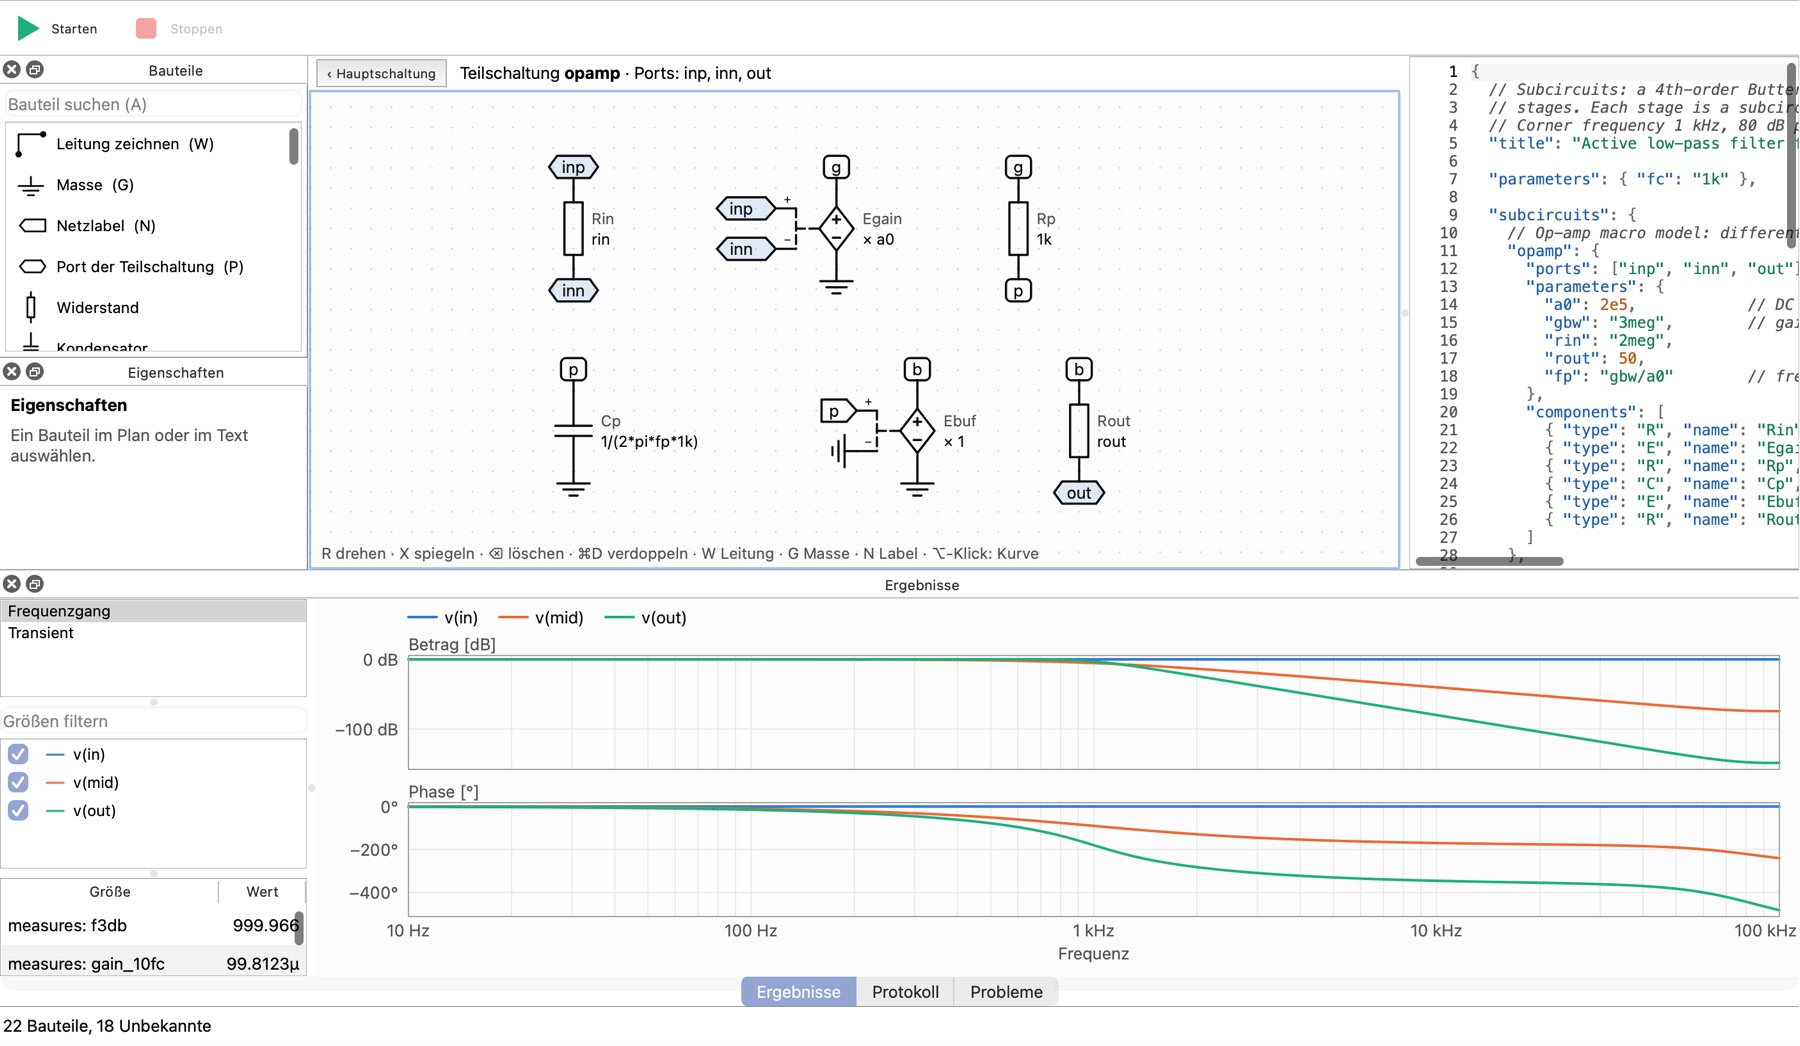
\includegraphics[width=\textwidth]{opamp_sub.jpg}
  \caption{Der Plan der Teilschaltung \code{opamp} aus
    \code{examples/opamp_filter.json}. Oben die Leiste mit dem Weg zurück
    und den Ports, im Plan die Ports \code{inp}, \code{inn} und \code{out}
    als beidseitig spitze Symbole.}
  \label{abb:opamp-sub}
\end{figure}

\section{Öffnen und zurück}

\begin{itemize}
  \item \textbf{Doppelklick} auf eine Instanz öffnet den Plan ihrer
    Teilschaltung (ebenso \menue{Teilschaltung „…“ öffnen} im
    Kontextmenü).
  \item Steht der Textcursor in einem Bauteil innerhalb einer
    Teilschaltung, wechselt der Plan von selbst dorthin.
  \item Über dem Plan steht dann eine Leiste: \menue{\guilsinglleft\ Hauptschaltung},
    der Name der Teilschaltung und ihre Ports.
  \item \menue{\guilsinglleft\ Hauptschaltung} oder \tasten{Strg}{$\uparrow$} führen zurück.
\end{itemize}

Im Plan einer Teilschaltung funktioniert alles wie in der Hauptschaltung;
dazu kommen die Ports.

\section{Ports}

Ein Port ist die Verbindung eines inneren Netzes nach außen. \taste{P} (oder
der Eintrag \menue{Port der Teilschaltung} in der Bauteilliste) fragt nach
dem Namen und setzt den Port per Klick. Ports verbinden wie Netzlabels über
ihren Namen.

\begin{itemize}
  \item Ein Port mit einem \emph{vorhandenen} Namen zeichnet einen Port der
    Teilschaltung an diese Stelle.
  \item Ein Port mit einem \emph{neuen} Namen erweitert die Ports: Der Name
    wird an \code{"ports"} angehängt, und jede Instanz bekommt einen
    Anschluss mehr (zunächst offen).
  \item Ports, die im Plan nicht gezeichnet sind, ergänzt der Editor am
    linken Rand.
\end{itemize}

\section{Eine neue, leere Teilschaltung}

\menue{Neue Teilschaltung \dots} in der Bauteilliste fragt nach dem Namen
und den Ports (durch Komma getrennt, z.\,B. \code{in, out, vdd}) und legt
unter \code{"subcircuits"} eine leere Definition an. Sie erscheint danach in
der Bauteilliste als »Teilschaltung „\textit{name}“« und wird wie jedes
andere Bauteil platziert. Ein Doppelklick auf die Instanz öffnet den noch
leeren Plan, in dem die Ports schon stehen.

\section{Auswahl in eine Teilschaltung umwandeln}
\label{sec:auslagern}

Aus einem Teil einer fertigen Schaltung wird so eine Teilschaltung:

\begin{enumerate}
  \item Die Bauteile im Plan auswählen (Rechteck aufziehen,
    Umschalt-Klick), samt ihrer Leitungen, Labels und Massen.
  \item \tasten{Strg}{G} drücken (oder \menue{In Teilschaltung umwandeln
    \dots} im Kontextmenü oder unter \menue{Bearbeiten}).
  \item Einen Namen für die Teilschaltung eingeben.
\end{enumerate}

Der Editor erledigt den Rest:

\begin{itemize}
  \item \textbf{Ports} werden die Netze, die Ausgewähltes mit dem Rest der
    Schaltung verbinden – von links nach rechts geordnet. Masse wird nie ein
    Port; sie ist überall dieselbe.
  \item Die \textbf{Grenze} liegt dort, wo ein nicht ausgewähltes Element
    ein ausgewähltes berührt. Innen sitzt dort der Port, außen ein Netzlabel
    mit dem Namen des Netzes, sodass alle Verbindungen erhalten bleiben.
  \item Die Bauteile wandern mit ihrem Text (Werte, Modelle, Kommentare)
    in die neue Definition, die Zeichnung mit ihnen.
  \item An ihrer Stelle steht eine Instanz mit Labels an den Anschlüssen.
\end{itemize}

Alles ist eine einzige Textänderung: \tasten{Strg}{Z} nimmt die ganze
Umwandlung in einem Schritt zurück. Die Schaltung rechnet vorher und
nachher dasselbe.

\section{Kurven und Spannungen in Teilschaltungen}

Im Plan einer Teilschaltung beziehen sich Kurven und Arbeitspunkt auf eine
Instanz. Ein \tasten{Alt}{Klick} auf das Netz \code{out} zeigt
\code{v(U1.out)}, wenn die Instanz \code{U1} heißt; ein Port steht für den
Knoten außen. Gibt es mehrere Instanzen, fragt der Editor, welche gemeint
ist. Die Spannungen an den Labels stehen nur, wenn die Teilschaltung genau
einmal verwendet wird.

Damit eine innere Größe als Kurve vorliegt, muss sie unter
\code{"outputs"} stehen (z.\,B. \code{"v(U1.mid)"}); die Statuszeile sagt,
was fehlt.

\section{SPICE-Teilschaltungen}

Teilschaltungen aus SPICE-Dateien (etwa Makromodelle von Operationsverstärkern
aus der Modellbibliothek) stehen als SPICE-Text in der Datei. Sie
erscheinen im Plan als Kasten mit den Ports der \code{.subckt}-Zeile, haben
aber keinen eigenen Plan: Ein Doppelklick zeigt ihren Text. Geändert werden
sie im Texteditor.
